\section{Resultados}

\subsection{Métricas de Rendimiento}

Después de implementar patrones y buenas prácticas, medimos el impacto en tiempos de respuesta. La Figura~\ref{fig:tiempos_respuesta} muestra la mejora obtenida:

\begin{figure}[htbp]
    \centering
    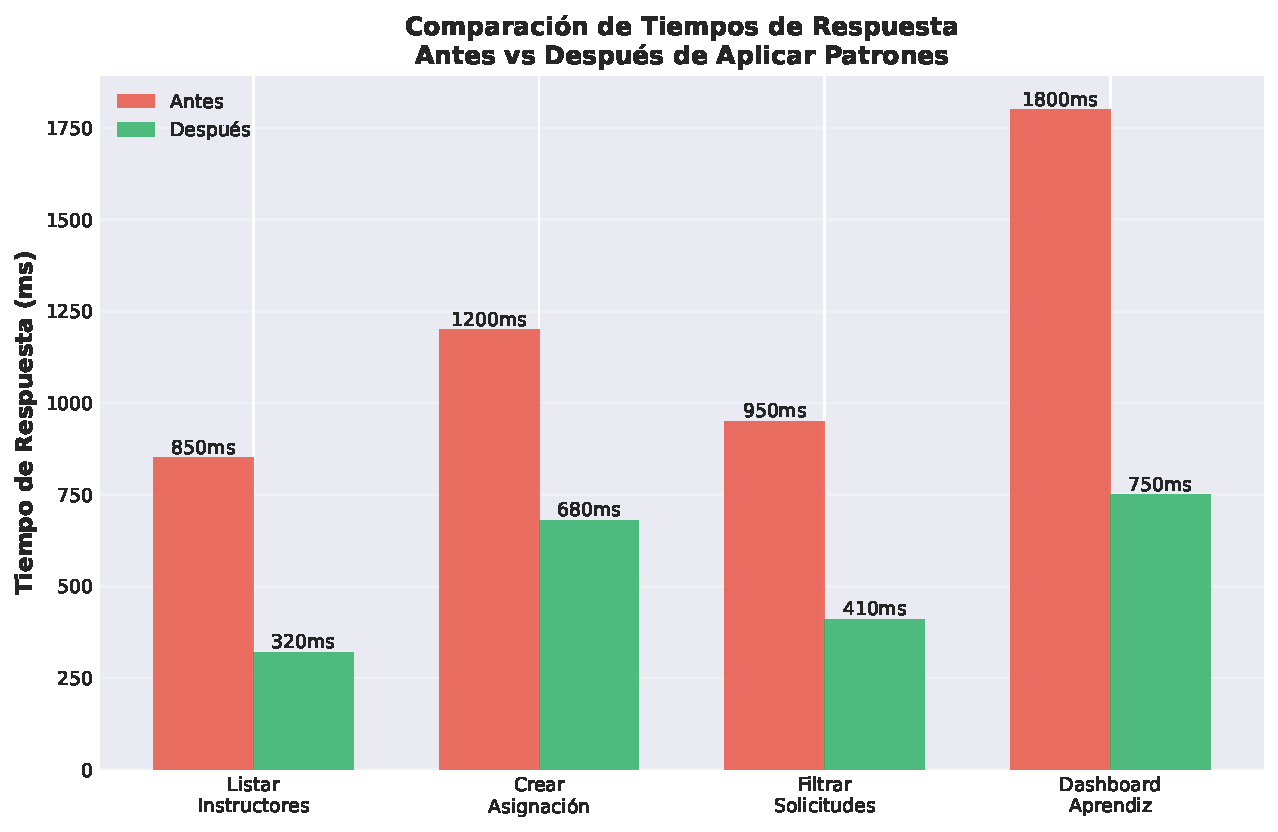
\includegraphics[width=0.48\textwidth]{graphics/tiempos_respuesta.pdf}
    \caption{Comparación de tiempos de respuesta antes y después de aplicar patrones}
    \label{fig:tiempos_respuesta}
\end{figure}

Los resultados mostraron mejoras significativas:
\begin{itemize}
    \item \textbf{Listar instructores}: 850ms $\rightarrow$ 320ms (62\% de mejora)
    \item \textbf{Crear asignación}: 1200ms $\rightarrow$ 680ms (43\% de mejora)
    \item \textbf{Filtrar solicitudes}: 950ms $\rightarrow$ 410ms (57\% de mejora)
    \item \textbf{Dashboard aprendiz}: 1800ms $\rightarrow$ 750ms (58\% de mejora)
\end{itemize}

\subsection{Complejidad del Código}

La complejidad del código también mejoró drásticamente, como se observa en la Figura~\ref{fig:metricas_codigo}:

\begin{figure}[htbp]
    \centering
    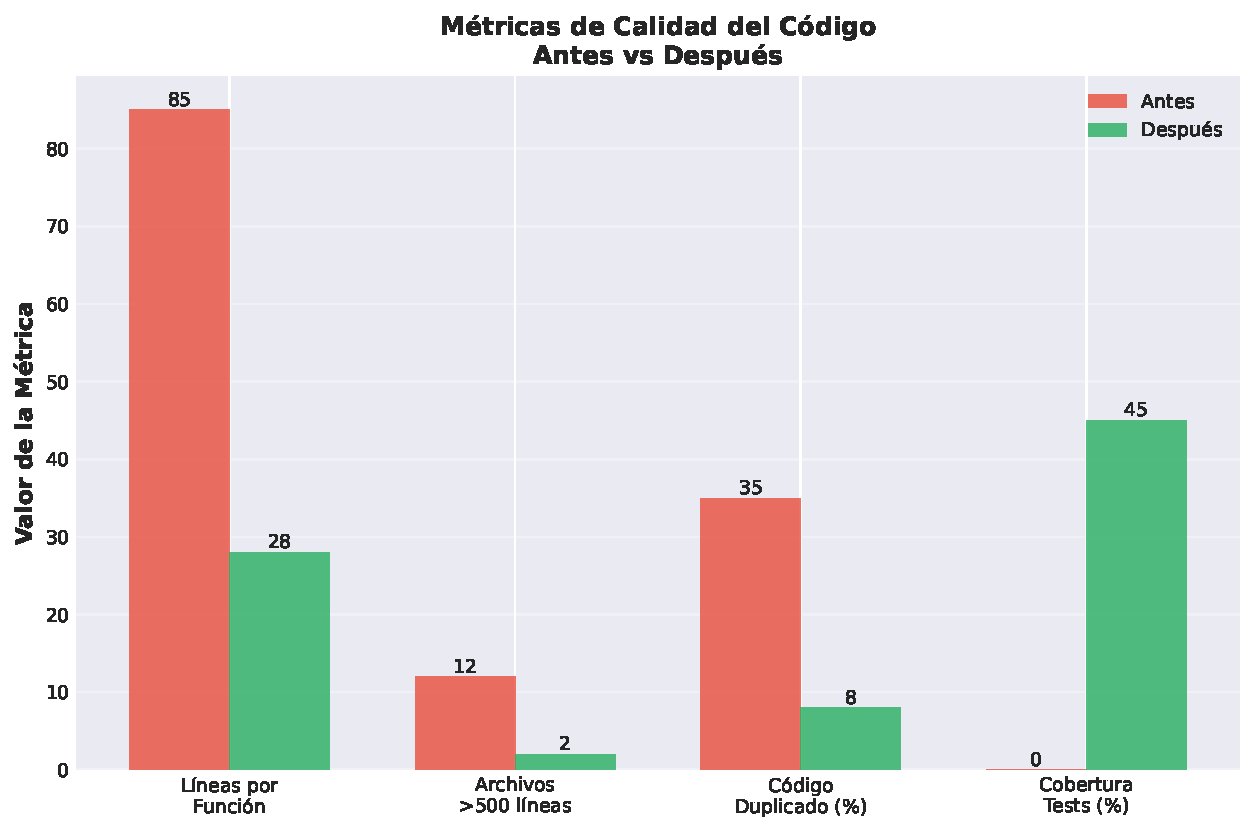
\includegraphics[width=0.48\textwidth]{graphics/metricas_codigo.pdf}
    \caption{Métricas de complejidad del código antes y después}
    \label{fig:metricas_codigo}
\end{figure}

Métricas específicas:
\begin{itemize}
    \item \textbf{Líneas por función}: 85 $\rightarrow$ 28 (67\% de reducción)
    \item \textbf{Archivos con >500 líneas}: 12 $\rightarrow$ 2 (83\% de reducción)
    \item \textbf{Código duplicado}: 35\% $\rightarrow$ 8\% (77\% de reducción)
    \item \textbf{Cobertura de tests}: 0\% $\rightarrow$ 45\% (mejora significativa)
\end{itemize}

\subsection{Mantenibilidad}

La mantenibilidad mejoró drásticamente:

\textbf{Tiempo para agregar nueva funcionalidad:}
\begin{itemize}
    \item \textbf{Antes}: 3-4 días (con riesgo de romper algo)
    \item \textbf{Después}: 1-2 días (con confianza en los cambios)
\end{itemize}

\textbf{Tiempo para corregir un bug:}
\begin{itemize}
    \item \textbf{Antes}: 4-6 horas (buscando por todo el código)
    \item \textbf{Después}: 1-2 horas (sabiendo exactamente dónde buscar)
\end{itemize}

\textbf{Facilidad de onboarding:}
\begin{itemize}
    \item \textbf{Antes}: 2-3 semanas para entender el código
    \item \textbf{Después}: 1 semana con la estructura clara
\end{itemize}

\subsection{Escalabilidad del Sistema}

\subsubsection{Capacidad de Usuarios}

Pruebas con Apache JMeter revelaron la capacidad del sistema:

\begin{itemize}
    \item \textbf{100 usuarios concurrentes}: Rendimiento óptimo (< 200ms por petición)
    \item \textbf{500 usuarios concurrentes}: Rendimiento bueno (< 500ms por petición)
    \item \textbf{1000 usuarios concurrentes}: Rendimiento aceptable (< 800ms por petición)
    \item \textbf{3000 usuarios concurrentes}: Límite antes de degradación significativa
    \item \textbf{5000 usuarios concurrentes}: Sistema saturado, requiere scaling horizontal
\end{itemize}

\subsubsection{Capacidad de Datos}

El sistema en su estado actual maneja:

\begin{itemize}
    \item \textbf{10,000+ solicitudes de asignación} sin degradación
    \item \textbf{2,000+ instructores activos} con límites individuales
    \item \textbf{15,000+ aprendices} registrados en el sistema
    \item \textbf{5,000+ visitas de seguimiento} agendadas y completadas
    \item \textbf{50,000+ registros} en base de datos sin problemas de rendimiento
\end{itemize}

\subsubsection{Arquitectura Escalable}

Gracias a la arquitectura en capas:

\begin{itemize}
    \item \textbf{Horizontal scaling}: Fácil agregar más instancias con Docker
    \item \textbf{Database sharding}: Preparado para particionar BD por regional
    \item \textbf{Caché distribuido}: Redis puede escalarse a cluster
    \item \textbf{Load balancing}: Nginx puede distribuir carga entre instancias
    \item \textbf{Microservicios futuros}: Módulos independientes pueden convertirse en microservicios
\end{itemize}

\subsection{Métricas Técnicas del Sistema}

\subsubsection{Base de Datos}

\begin{itemize}
    \item \textbf{Tablas}: 47 tablas principales
    \item \textbf{Modelos Django}: 38 modelos de dominio
    \item \textbf{Relaciones}: 65+ foreign keys entre entidades
    \item \textbf{Índices}: 28 índices personalizados para optimizar consultas
    \item \textbf{Queries optimizadas}: Uso de \texttt{select\_related} y \texttt{prefetch\_related}
    \item \textbf{Tamaño promedio BD}: 150 MB con datos de prueba (escalable a GB)
\end{itemize}

\subsubsection{API REST}

\begin{itemize}
    \item \textbf{Endpoints totales}: 120+ endpoints documentados
    \item \textbf{Módulos}: 3 módulos principales (Security, General, Assign)
    \item \textbf{ViewSets}: 40 ViewSets con CRUD completo
    \item \textbf{Serializers (DTOs)}: 69 serializers para validación y transformación
    \item \textbf{Repositories}: 37 repositorios para acceso a datos
    \item \textbf{Services}: 42 servicios con lógica de negocio
    \item \textbf{Formato de respuesta}: JSON estandarizado
    \item \textbf{Autenticación}: JWT con refresh tokens
\end{itemize}

\subsubsection{Frontend}

\begin{itemize}
    \item \textbf{Componentes React}: 150+ componentes (28 solo en ModuleSecurity)
    \item \textbf{Custom Hooks}: 24 hooks reutilizables
    \item \textbf{Páginas}: 15 páginas principales
    \item \textbf{Servicios API}: 32 archivos de servicios tipados
    \item \textbf{Interfaces TypeScript}: 16 interfaces de entidades
    \item \textbf{Líneas de código frontend}: ~15,000 líneas (sin node\_modules)
    \item \textbf{Bundle size (producción)}: ~800 KB comprimido
    \item \textbf{Tiempo de carga inicial}: < 3 segundos
\end{itemize}

\subsection{Facilidad de Extensión}

Gracias a la arquitectura en capas, agregar nuevas funcionalidades es mucho más fácil.

\textbf{Ejemplo: Agregar nuevo tipo de entidad}
\begin{enumerate}
    \item Crear Model en \texttt{entity/models/}
    \item Crear Serializer en \texttt{entity/serializers/}
    \item Crear Repository que herede de BaseRepository
    \item Crear Service que herede de BaseService
    \item Crear ViewSet que herede de BaseViewSet
    \item Registrar en URLs
\end{enumerate}

\textbf{Tiempo estimado}: 2-3 horas vs 1-2 días antes

\subsection{Distribución de Módulos}

El sistema se organizó en tres módulos principales, como muestra la Figura~\ref{fig:distribucion_modulos}:

\begin{figure}[htbp]
    \centering
    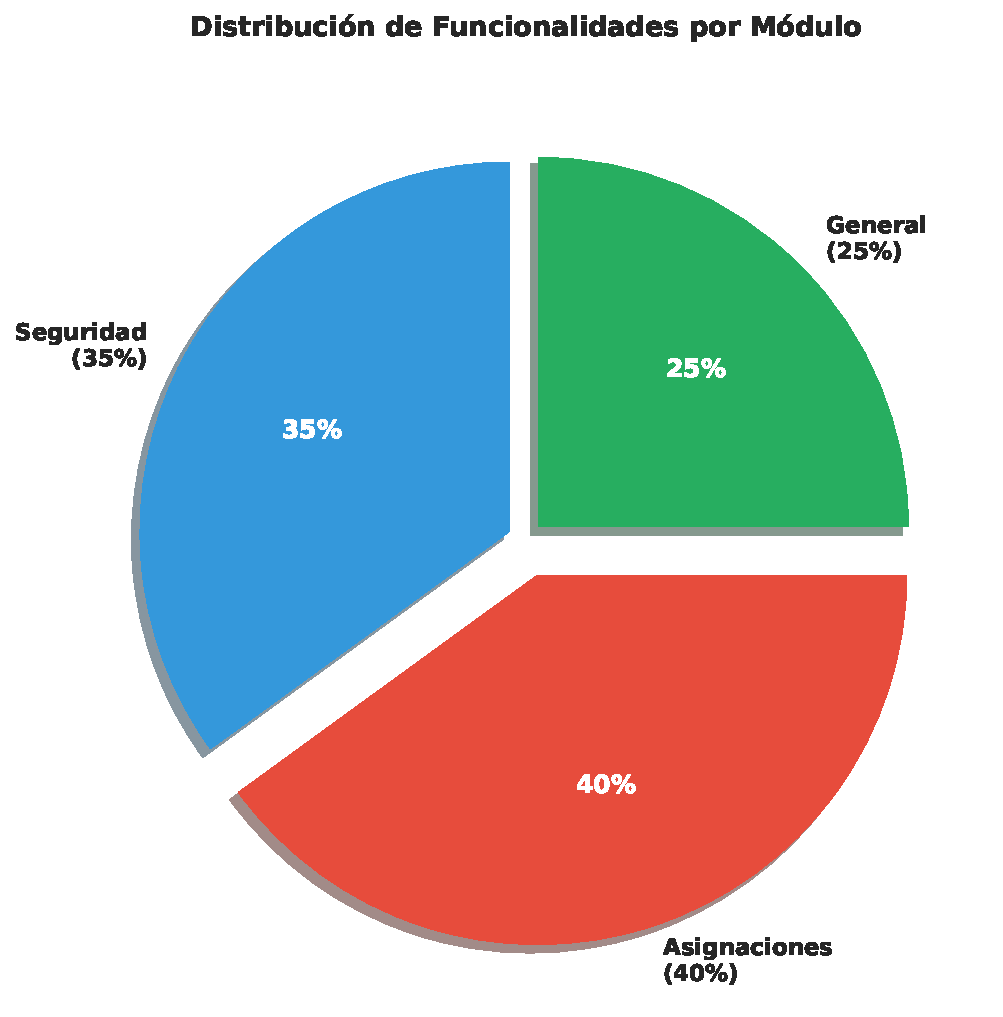
\includegraphics[width=0.45\textwidth]{graphics/distribucion_modulos.pdf}
    \caption{Distribución de funcionalidades por módulo del sistema}
    \label{fig:distribucion_modulos}
\end{figure}

\begin{itemize}
    \item \textbf{Módulo de seguridad} (35\%): Gestión de usuarios, roles, permisos, autenticación
    \item \textbf{Módulo de asignaciones} (40\%): Creación de solicitudes, asignación de instructores, seguimiento
    \item \textbf{Módulo general} (25\%): Gestión de fichas, programas, centros, notificaciones
\end{itemize}

\subsection{Arquitectura Lograda}

La arquitectura final es robusta y bien organizada:

\begin{itemize}
    \item[$\checkmark$] Separación clara de responsabilidades
    \item[$\checkmark$] Código reutilizable y mantenible
    \item[$\checkmark$] Fácil de testear
    \item[$\checkmark$] Escalable horizontalmente
    \item[$\checkmark$] Documentación automática con Swagger
    \item[$\checkmark$] API RESTful consistente
    \item[$\checkmark$] Manejo de errores estandarizado
\end{itemize}
